\chapter{Calculational tools}
\label{ToolsAppendix}
\graphicspath{{Figures/ToolsAppendix/}{Figures/Common/}}

Although not theoretical physics of itself, a not insignificant part of any theoretical physics work is spent in the technical task of using computational tools.  It is unsurprising therefore that just as experimental PhD candidates will spend a significant portion of their time building and designing the apparatus for experiments, so too will a theorist spend time developing the codes that they need in the pursuit of their work.  In this appendix I describe the tool that I have developed in the course of my PhD to simplify the process of developing these codes.  %I would like to think that the work described here might be used beyond the term of my PhD and more widely than by myself. more widely find wider application beyond wider application

\parasep

A wide variety of simulations have been necessary in pursuit of the goals of this thesis.  These have included simulations for the calculation of condensate ground states, the propagation of both Gross-Pitaevskii and Truncated Wigner atom laser models of different atomic species in systems of different dimensionality, the evolution of matrices describing quasiparticles, the evolution of a variety of optical pumping models, and the evolution of an evaporation-driven pumped atom laser.  With the exception of the last of these simulations, which was written by \emph{Matthew Davis}, all of these simulations have been written by myself.  The work necessary to hand-write all of these codes from scratch would have been prohibitive.  Each would have needed independent testing, and the associated time fixing errors.  Instead, codes for almost all of the simulations in this thesis were produced by the computational package \XMDS\ \citep{Collecutt:2001}, or its successor, \xpdeint.  Each of these tools take a high-level description of a problem (an input script) and produce a fast low-level simulation (written in \texttt{C++}) that solves the problem.  By testing these packages extensively, the common aspects of simulations can be generated reliably.

A large number of problems solved within the fields of quantum and atom optics are very similar on a mathematical level as they fall into the class of systems of initial-value (stochastic) partial differential equations.  Due to the similarity of problems of this form, it is feasible to create a packages such as \XMDS\ and \xpdeint\ which focus purely on solving this type of problem.  These problems can also be solved with more general purpose tools like \texttt{MATLAB} and \texttt{Mathematica}, and these tools are ideal when the problem is sufficiently small that it may be solved with their built-in integrators.  However, when the problem becomes sufficiently large that the overheads of these tools become significant, traditionally a hand-coded solution has been necessary.  \XMDS\ and \xpdeint\ provide an alternative to writing such codes by hand.

\XMDS\ and \xpdeint\ particularly excel at providing a smooth transition from a low-dimensional simulation to a higher-dimensional one, from a deterministic simulation to a stochastic one, or from a single-processor simulation to a distributed simulation running in parallel across multiple computers.  In hand-written codes, unless they were initially written with such a potential future extension in mind, each such change would require significant effort in rewriting the code.  In \XMDS\ and \xpdeint, such changes require only minimal change to the input script.  This encourages users to create test simulations of a simpler system (e.g.\ reduced dimensionality), which makes the code run faster, allowing problems in the input script to be found and fixed more quickly.  Later, the simulation can be scaled up to the full problem.  Fundamentally, the ease with which codes can be generated encourages \emph{experimentation} with different types of simulations, as the time taken to create the code is no longer the rate-limiting factor.  FIXME: Note that it is not my intent that simulation replace analytical work, I hope that I have demonstrated the importance of estimations and approximations in this thesis.  Instead, the advantage of \XMDS\ and \xpdeint\ is in simplifying the process once it has been determined that a simulation is necessary.  ``A computation is a temptation that should be resisted as long as possible'' --- J.P.~Boyd, paraphrasing T.S.~Eliot \citep{SpectralMethods}.

\XMDS\ was originally created in 2001 by \citet{Collecutt:2001}, and has been improved over the intervening years by a large number of contributors (including myself) adding a variety of integrators, interaction picture algorithms \citep{Caradoc-Davies:2000qy}, cross-propagation algorithms, and the ability to solve deterministic problems in parallel.  Over this period of time, \XMDS\ has been employed for wide range of problems, including quantum optical information storage in two-level atoms \citep{Hetet:2008}, the influence of mobility on biodiversity \citep{Reichenbach:2007}, polarisation squeezing in optical fibres \citep{Corney:2006}, and quantum superchemistry in molecular Bose-Einstein condensates \citep{Hope:2001a}\footnote{FIXME: If anyone has a favourite interesting application of \XMDS\ that isn't in this list, let me know and I'll add it.}.  

Since the development of \XMDS, there have been other problems to which it has been desired to apply \XMDS, but as it was not designed with such systems in mind, either less-than-satisfactory solutions were used, or a separate code was written by hand.  A good example of such problems were simulations involving cylindrical or spherical symmetry.  As \XMDS\ calculates spatial derivatives using Fourier transforms, the solution is necessarily assumed to be periodic over the computational domain.  This is a complication when it is desired to use cylindrical or spherical symmetry as the solution near the origin is not necessarily similar in value to the solution at the outer edge of the computational domain.  This problem has been resolved by including an unphysical negative range to the radius (for example, this technique was used in \citep{Wuster:2005,Dall:2009}).  This solution is unsatisfying as it increases by at least a factor of 2 the computational resources required the solve the problem, reduces the order of convergence of the solution (when considered as a function of the number of spatial grid points used), and care must be taken in the choice of the grid to exclude the origin as a point.  This step is necessary as the Laplacian operator in cylindrical and spherical coordinates contains terms involving inverse powers of the radius.  Were the origin included as a point in the computational grid, it would be necessary to divide by zero.

The actual motivation for the creation of a successor to \XMDS\ was the need for an algorithm to solve the optical pumping model \eqref{OpticalPumping:GeneralMultimodeModel}, specifically an algorithm which could solve partial differential equations in time coupled with auxiliary equations which propagate in space in \emph{opposite} directions.  A specific example of such a system is the $2 \hbar k$ momentum transfer `simple atom laser model' of \sectionref{OpticalPumping:SimpleModels:AtomLaserModel}.  \XMDS\ implements an algorithm that can solve such auxiliary equations when they propagate in a single direction.  This `cross-propagation' algorithm needed to be extended to implement the Alternating-Direction Implicit algorithm \citep{NumericalRecipes}, which can handle the more general case.  While this algorithm could have been implemented in \XMDS, it would have required significant effort as although \XMDS\ was a powerful tool, its internal workings had become somewhat of a tangled mess that worked more through the sheer effort of those who modified it than because it was designed in such a way as to make any extensions require an appropriate amount of effort.  Nevertheless, the effort necessitated in adding features to \XMDS, without a doubt, saved more effort overall for \XMDS's users.  

I felt that a rewrite of \XMDS\ could not only address my specific problem and other limitations (such as those that arise when dealing with problems with cylindrical or spherical symmetry), but could make it easier to extend in the future.  This was no minor task as \XMDS\ contained approximately 38000 lines of code.  While none of \XMDS's code could be directly copied, the parts implementing the various integrators could be translated fairly simply, and some of the ideas in \XMDS\ could be directly implemented in \xpdeint, making the rewrite a slightly less daunting task.  The current version of \xpdeint\ (at the time of printing) contains approximately 22000 lines of code, and implements almost all of the features of \XMDS, while also improving upon it in several key areas.  The features of \xpdeint\ are the subject of the remainder of this appendix.

\section{\xpdeint}

% \begin{figure}
%     \centering
%     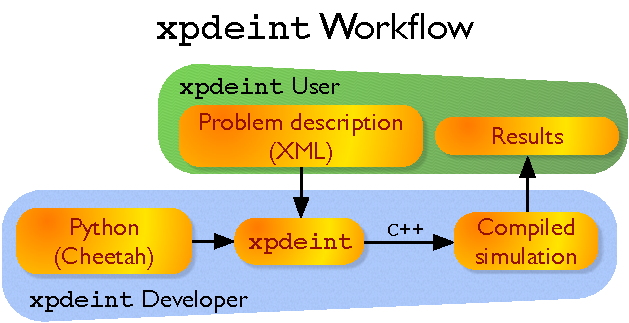
\includegraphics[width=10cm]{xpdeintWorkflow}
%     \caption{FIXME: This is not a caption.\label{ToolsAppendix:xpdeintWorkflow}}
% \end{figure}

As discussed in the previous section, the class of problem that can be solved with \xpdeint\ (and \XMDS) is that of systems of initial-value (stochastic) partial differential equations.  To solve such problems numerically, they must be restricted to a finite domain with boundary conditions imposed at the edges.  \xpdeint\ discretises this problem by applying the pseudo-spectral method \citep{SpectralMethods}: the solution is decomposed as a weighted sum of a finite set of basis functions,
\begin{align}
    f(x) &= \sum_{n=1}^{N} c_n g_n(x),
\end{align}
where $f(x)$ is the spatial representation of the solution, $g_n(x)$ are the basis functions, and $\{c_n\}$ are constants which form an equivalent representation of the solution (the \emph{spectral} representation \citep{SpectralMethods}).  The choice of basis functions is significant as it determines the boundary conditions at the edge of the computational domain, and some sets of basis functions are more appropriate for some problems than others.  

The most common problem that \xpdeint\ is applied to is the solution of Schrödinger-like equations.  For such problems, the potential and $s$-wave scattering terms are local in the spatial representation, and are therefore accurately calculated with any set of basis functions.  The kinetic energy term, being proportional to the Laplacian operator, does not share this property as knowledge of the solution in the region near a point is necessary to evaluate it.  By choosing the basis functions to be the eigenfunctions of the Laplacian operator, the kinetic energy may be evaluated more accurately in the spectral representation.  For example,
\begin{align}
    \frac{- \hbar^2 \nabla^2}{2 M} f(x) &= \frac{-\hbar^2}{2 M}\sum_{n=1}^{N} \lambda_n c_n g_n(x),
\end{align}
where $\lambda_n$ is the eigenvalue for the Laplacian eigenfunction $g_n(x)$, i.e.\ $\nabla^2 g_n(x) = \lambda_n g_n(x)$.  \xpdeint\ implements a range of different types of basis functions for use in problems exhibiting different types of symmetries: the Fourier basis for translation-invariant problems, the sine and cosine bases for problems with reflection symmetry, the Bessel and spherical-Bessel bases for problems with cylindrical and spherical symmetry, and the Hermite-Gauss basis where the basis functions are the harmonic oscillator eigenstates.  This last basis is useful in (stochastic) projected-GP models in which it permits an implementation of a self-consistent energy cut-off \citep{Blakie:2008a}.  Of these different types of bases, only the first, the Fourier basis, was available in \XMDS.  The advantage of the Fourier basis is that it permits the use of the Fast Fourier Transform (FFT), a `fast' algorithm ($O(N \log N)$ operations for an $N$-point 1D Fourier transform) for transforming between the spatial and spectral representations.  Similar algorithms may also be used for the sine and cosine bases, but all other bases require the use of a matrix multiplication to transform between the spatial and spectral representations.  In contrast, matrix multiplication requires $O(N^2)$ operations for an $N$-point 1D transform.  In practice, this cost can be reduced by a factor of two when every basis function has a definite parity (i.e.\ even or odd with respect to the origin, an example is the Hermite-Gauss basis), and such an algorithm is implemented in \xpdeint.  Although the matrix multiplication transform is slower than the FFT, for sufficiently small numbers of grid points ($\lesssim 100$), the cost is not significantly larger, and may be outweighed by the better convergence afforded by using a more appropriate set of basis functions.

The details of pseudo-spectral methods and their implementation via Gaussian quadrature are beyond the scope of this appendix, our purpose here has been to give an overview of the technique.  The topic is discussed in significant depth elsewhere \citep{SpectralMethods}.

Keep in mind the dipole--dipole interaction.  This term is not local in position space... but is local in Fourier space?
For such problems, the potential terms are typically local, and special care must be taken of the kinetic energy operator

FFTW3: \citep{Frigo:2005}.

While none of the techniques described in this appendix are new, the utility of \xpdeint\ is the ease with which such a wide range of algorithms and methods can be applied.  While the generality cannot be compared with such tools as MATLAB and Mathematica, the advantage is in the focussed design and speed advantages (for large problems).

\begin{itemize}
    \item A variety of (mostly explicit) integrators
    \item Spectral method
    \item IP operator
    \item Various basis functions (sine/cosine/Fourier/Bessel/Spherical Bessel/Hermite-Gauss) faster PMMT transform used where possible.
    \item Coupled ODE-PDE systems
    \item Gaussian quadrature
    \item Stochastic integration (Gaussian and/or Poissonian noises)
    \item Distributed simulations
    \item (Multi-dimensional multi-directional) Cross-propagation
    \item Tensor-valued equations (although not with very nice notation)
    \item Convolutions
    \item Non-local access (ability to calculate correlation functions)
    \item Generates faster code than xmds
    \item More descriptive errors
    \item More portable output format (HDF5)
    \item Diagnostics
\end{itemize}

Things \xpdeint\ has been used for: the calculation of Lyapunov exponents in classical/semiclassical systems, control of a BEC, new and interesting stochastic phase-space methods, molecular disassociation, soliton dynamics, stuff.

Papers that use \xpdeint: \citet{Doring:2009,Szigeti:2009,Hush:2009,Hush:2010}.